\documentclass[10pt,a4paper]{article}
\usepackage[T1]{fontenc}
\usepackage[a4paper]{geometry}
\usepackage{xcolor}
\usepackage{amssymb}
\usepackage{amsmath}
\usepackage{graphicx}
\usepackage{tabularx}
\usepackage{multirow}
\usepackage{subfigure}
\usepackage{verbatim}
\usepackage{fancyhdr}
\usepackage{listings}
\usepackage{../common/espacs}

%\input{../common/commands.tex}

\title{Exercise Session 4}
\date{October 26, 2012}

\pagestyle{fancy}
\headheight 35pt

\rhead{\copyright~2006/2012}

\newcommand{\vv}[1]{\mathbf{#1}}

\begin{document}
\lstset{language=[ISO]C++}
\maketitle

\section*{Google PageRank}

Dalla sua nascita, Google ha impiegato brevissimo tempo per imporsi
come il pi\`u utilizzato motore di ricerca rispetto a tutti i
concorrenti. Il successo \`e dipeso dalla accuratezza delle risposte,
molto superiore a quelle di altri motori di ricerca.
Google infatti stila una propria classifica (\emph{ranking})
dell'importanza delle pagine web, per ordinare i risultati proposti;
molto spesso questa classifica \`e proprio quella desiderata l'utente.

L'algoritmo che ordina le pagine web per importanza \`e denominato
\emph{PageRank} ed \`e stato sviluppato da S.~Brin e L.~Page presso
la Stanford University \cite{Brin1998}.
Il principio su cui si basa \`e il seguente:
\begin{itemize}

    \item se una pagina web A ha un collegamento (\emph{link}) verso una
        pagina B, questo \`e interpretato come un voto di A in favore di B
        (cio\`e alza B in graduatoria);

    \item i votanti non sono tutti uguali: il voto di chi \`e alto in
        classifica (cio\`e ha ricevuto molti link) vale maggiormente di quello di chi \`e
        in basso.

\end{itemize}

\begin{figure}[htbp]
    \centering
    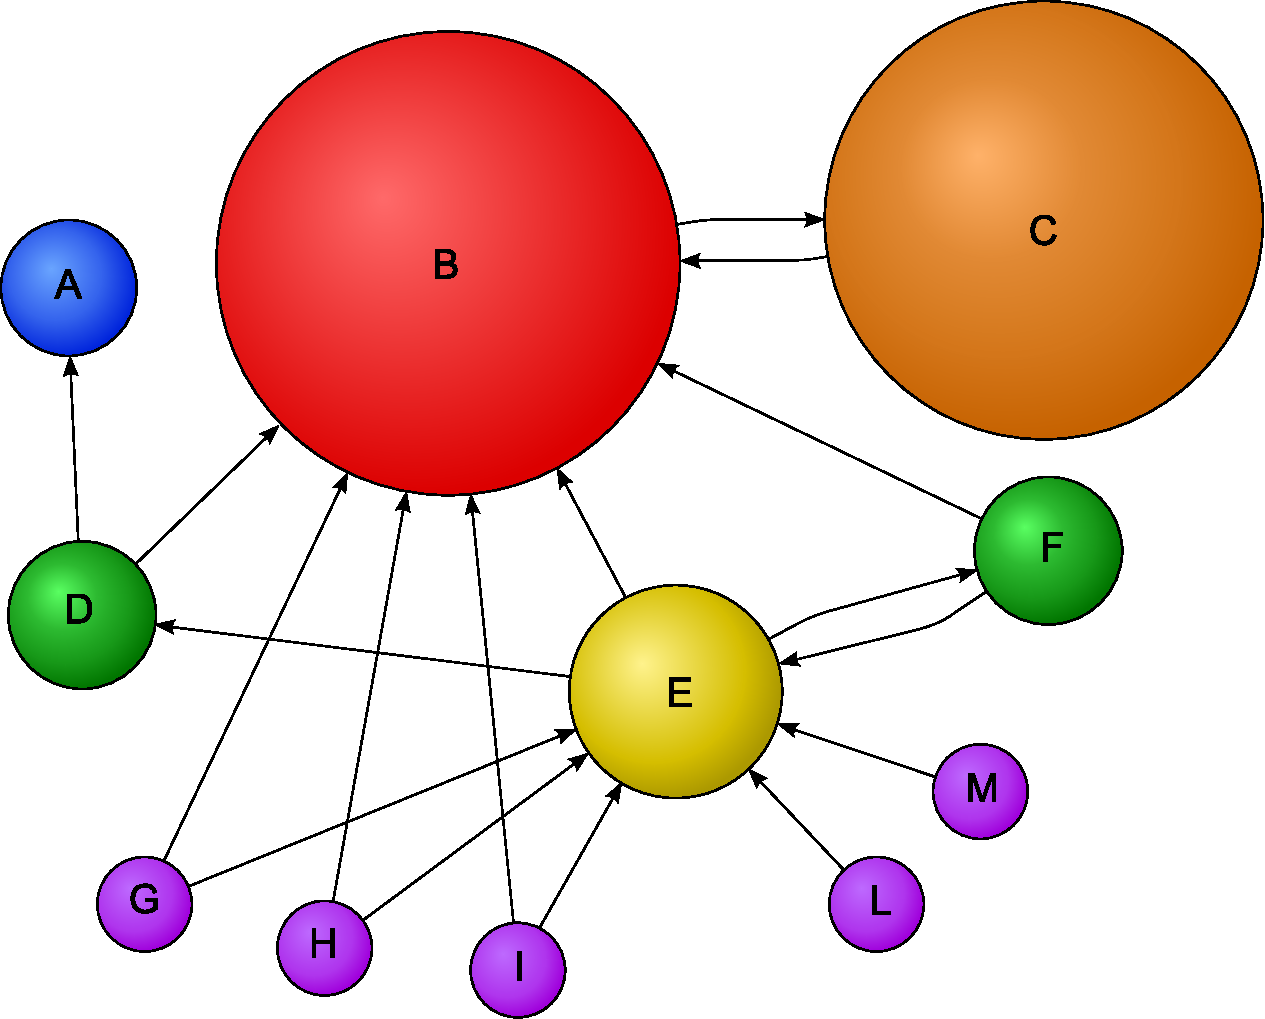
\includegraphics[width=0.6\textwidth]{./fig/PageRanks_Example_only_letters}
    \caption{Diagramma schematico del \emph{ranking}: ogni sfera rappresenta una pagina
            web, ogni freccia un link, la dimensione delle sfere \`e l'importanza
            attribuita alla pagina.}\label{fig:PR}
\end{figure}


Questo principio \`e descritto schematicamente in Fig.~\ref{fig:PR}.
La pagina B riceve molti link e quindi \`e considerata molto importante. La pagina
C \`e considerata pi\`u importante di E, anche se riceve meno link, perch\`e il voto di
B conta molto di pi\`u dei tanti ``piccoli'' voti che riceve E
(ad es. se il ``Washington Post'' o il ``New York Times'' pubblicassero un link al sito
web di ``Programmazione Avanzata per il Calcolo Scientifico'' questo varrebbe
molto di pi\`u dei link dai siti web personali di docente, esercitatore e studenti del corso!).

Dal punto di vista formale, si definisce il \emph{ranking} (importanza relativa) $r(p)$
della pagina $p$ come la somma di tutti i \emph{ranking} $r(q)$ di tutte le
pagine $q$ che puntano $p$:
\begin{align}
    \label{eq:rank}
    r(p)=\sum_{q \rightarrow p} \frac{r(q)}{\#q};
\end{align}
la somma \`e ponderata da $\#q$, numero di link presenti nella pagina $q$
(se una pagina $q$ ha un solo link verso $p$ \`e probabile che un lettore interessato lo segua,
viceversa se la pagina $q$ ha moltissimi link \`e poco probabile che il lettore scelga
proprio quello verso $p$).
\`E facile notare che si tratta di un problema in forma implicita: per conoscere il ranking di
$p$ si devono conoscere quelli delle altre pagine, che a loro volta si basano su quello di $p$.

Fortunatamente il problema \`e affrontabile in modo relativamente semplice, una volta scritto
in forma matriciale. Siano $\{p_1, p_2, \dots p_N\}$ tutte le pagine web censite e sia
$A \in \mathbb{R}^{N \times N}$ la matrice di connessione, il cui elemento $a_{i,j}$ \`e dato da:
\begin{align}
      \label{eq:harmonicp}
      a_{i,j}=
      \begin{cases}
        \dfrac{1}{\#p_j} &\qquad \mbox{se esiste un link da $p_j$ a $p_i$} \\[5mm]
        0 & \qquad \mbox{altrimenti.}
      \end{cases}
\end{align}

Si noti che gli $a_{i,j}$ possono essere intepretati come una distribuzione di probabilit\`a,
in particolare rappresentano la probabilit\`a che un persona che clicca a caso giunga alla
pagina $p_i$ a partire dalla pagina $p_j$. La matrice gode della propriet\`a:
\begin{align} \label{eq:sum1}
    \sum_{i=1}^{N} a_{i,j}=1.
\end{align}

Se il \emph{ranking} delle pagine web $p_i$ \`e rappresentato dal vettore colonn
\emph{PageRank} $\vv{r}=[r_1,r2, \dots r_n]^T$, allora l'equazione \eqref{eq:rank}
equivale al seguente problema:
\begin{align*}
    \vv{r}=A \vv{r}.
\end{align*}
Il \emph{PageRank} \`e quindi l'autovettore corrispondente all'autovalore 1 del problema
agli autovalori associato. Si pu\`o dimostrare che se i $\lambda_i$ sono gli autovalori
di $A$ allora $|\lambda_i| \leq 1$. Inoltre $\lambda_1=1$ ha molteplicit\`a
uno\footnote{Una condizione sufficiente \`e fornita dal teorema di Perron Frobenius,
che richiede una matrice corrispondente ad un grafo irriducibile. Un trucco per
soddisfare l'ipotesi potrebbe essere quello di attribuire un link ad ogni pagina
esistente alle pagine senza link.}.

Dato che il numero di pagine censite $N$ \`e dell'ordine di grandezza delle decine di
miliardi, il calcolo con un metodo diretto dell'autovettore \emph{PageRank} \`e
computazionalmente troppo oneroso, anche per chi dispone di risorse di calcolo eccezionali.
Si utilizza quindi un metodo iterativo, che restituisce una soluzione approssimata,
ad esempio ci si potrebbe basare sul metodo delle potenze. In questo caso particolare,
arrestare il numero di iterazioni al passo $k$ significa aver considerato solo le pagine
$p_j$ che distano da $p_i$ al pi\`u $k$ click\footnote{Per ragioni di semplicit\`a di
esposizione tralasciamo la possibilt\`a di introdurre un fattore di rilassamento
(\emph{damping fatctor}) \cite{Brin1998}, che comunque non modifica il principio base
dell'algoritmo.}.

\subsection*{Metodo delle potenze}

Il \emph{metodo delle potenze} \`e applicabile a matrici in cui
l'autovalore di modulo massimo $\lambda_1$ abbia molteplicit\`a
unitaria e sia ben separato dall'autovalore immediatamente pi\`u
piccolo in modulo. Il generico passo dell'algoritmo \`e riportato di
seguito:
\begin{align*}
    {\bf q}\iter{k} &= \frac{ A{\bf q}\iter{k-1} }{
        \norm{ A{\bf q}\iter{k-1}}_2 },\\
    {\bf \nu}\iter{k} &= {{\bf q}\iter{k}}^T  A {\bf q}\iter{k},\\
    {\bf w}\iter{k} &= \frac{ {{\bf w}\iter{k-1}}^T A }{
        \norm{ {{\bf w}\iter{k-1}}^T A}_2 },
\end{align*}
dove con $\nu\iter{k}$, ${\bf q}\iter{k}$ e ${\bf w}\iter{k}$ si sono
indicate, rispettivamente, le approssimazioni di $\lambda_1$ e degli
autovalori destro e sinistro ${\bf x}_1$ e ${\bf y}_1$ ad esso
associati. Vale la seguente stima, utile per determinare un criterio
d'arresto:
\begin{align*}
    \module{ \lambda_1 - \nu\iter{k} } \approx %
    \frac{ \norm{ {\bf r}\iter{k} }_2 }{
    \module{ {{\bf w}\iter{k}}^T \cdot{\bf q}\iter{k} } },
\end{align*}
dove ${\bf r}\iter{k} \eqbydef A{\bf q}\iter{k} - \nu\iter{k}{\bf
q}\iter{k}$ \`e il residuo all'iterazione $k$-esima.

\subsection*{Libreria di algebra lineare: Eigen}

La codifica dei metodi per il calcolo degli autovalori di una matrice
richiede una libreria per la gestione dell'algebra
lineare. La libreria di algebra lineare proposta e utilizzata
nel corso \`e Eigen versione 3.0.
Tale libreria permette di gestire in maniera efficiente sia
matrici sparse che matrici piene.


\subsection*{Exercise 1}

Build the connection matrix $B\in \mathbb{R}^{5 \times 5}$ relative to the web
made of the 5 pages, as depicted in Fig.~\ref{fig:web}.
%
\begin{figure}
\centering
\includegraphics[width=0.4\textwidth]{fig/tikz/pagerank5}
\caption{Scheme for a 5 pages web. Every circle is a page, every arrow is a
link.}
\label{fig:web}
\end{figure}
%
Using the \texttt{Eigen} library, write down a class that computes the maximum
eigenvalue (that is 1) and the corresponding eigenvector, that is the
\emph{pagerank}. Implement also \cpp{operator<<} to see the data inside the
class on the screen.

\subsection*{Solution}

The proposed solution implements the power method using vectors and matrices
from the \texttt{eigen} library.

The class \cpp{LinearAlgebra::Eigenvalues::PowerMethod} has one constructor
that takes as parameters the tolerance and the max iteration number. We set
a max iteration number in order to avoid an infinite loop when there is no
convergence. The power method is applied with a call to the \cpp{apply} method,
that requires the matrix and an approximation of the right eigenvector as
input. The code uses this approximation also as seed for the left eigenvector.
The code for the \cpp{Power} class is as follows
%
\lstset{basicstyle=\scriptsize\sf}
    \lstinputlisting[caption=\cpp{Power} class interface]
    {./src/pagerank-eigen/src/power.hpp}
\lstset{basicstyle=\sf}

Note the two public \cpp{typedef}s at the beginning of the class. They can be
very useful from outside the class, since changing them inside the class updates
automatically all the code. It is interesting to compare the two implementations
for the \cpp{tol} and \cpp{maxit} methods. When there is a \cpp{const} keyword
at the end of the definition, it means that the method is intended to be just
for access. When there is no \cpp{const} keyword, the method is instead used to
modify the value of the private member. The copy constructor and the assignment
operator have the keyword \cpp{delete}, this means that the compiler is now
allowed to instantiate them implicitly. This way of disabling implicit
implementations is only available with \texttt{c++11}. If the new standard is
not available, a common way to avoid implicit instantiations is to declare the
method in the private section of the class and not implement it. this will raise
a compile error if the method is requested somewhere.

\lstset{basicstyle=\scriptsize\sf}
    \lstinputlisting[caption=\cpp{Power} class implementation]
    {./src/pagerank-eigen/src/power.cpp}
\lstset{basicstyle=\sf}

At the beginning of the \cpp{apply} method it is interesting to note the use of
two different constructors for \texttt{eigen} vectors. In the first and third
case the copy constructor is used, while on the second and forth case we use the
constructor that builds an empty vector of size \cpp{N}.

The listing for the \cpp{main} program follows
\lstset{basicstyle=\scriptsize\sf}
    \lstinputlisting[caption=Main program]
    {./src/pagerank-eigen/eig.cpp}
\lstset{basicstyle=\sf}

We note the use of the \cpp{typedef}s that come from the \cpp{PowerMethod}
class. They are accessed from outside the class with their fully specialized
name, with a syntax similar to the one used for namespaces. It is worth noting
that the use of the typedefs does not require the creation of an object of type
\cpp{PowerMethod}, just like the use of static functions and members does not
too.



\bibliographystyle{siam}
%\bibliography{../common/bibliography}

\begin{thebibliography}{9}

\bibitem{Brin1998} S.~Brin and L.~Page,
The anatomy of a large-scale hypertextual web search engine,
{\em Computer Networks and ISDN Systems}, vol.~30, no.~1-7, pp.~107 -- 117,
1998. Proceedings of the Seventh International World Wide Web Conference.

\end{thebibliography}

\end{document}
